\documentclass[12pt, a4paper]{article}

\usepackage{amsmath}
\usepackage{amsfonts}
\usepackage{amssymb}
\usepackage{graphicx}
\usepackage{float}
\usepackage{listings}
\usepackage{rotating}
\usepackage{tikz}
\usepackage{verbatim}
\pdfgentounicode=1
\pdfmapline{+cyberb@Unicode@  <cyberbit.ttf}

\begin{document}

\title{XXX}
\author{P. Baillehache}
\date{\today}
\maketitle

\tableofcontents

\section*{Introduction}

JSCarousel is a JavaScript library to create a carousel of pictures on a webpage.\\

You can have a look at JSCarousel here: http://www.bayashiinjapan.net/Carousel01/\\

JSCarousel has one external dependancy: JQuery which can be found here: https://jquery.com/download/\\

\section{jscaroussel.js}

\begin{scriptsize}
\begin{ttfamily}
\verbatiminput{../jscaroussel.js}
\end{ttfamily}
\end{scriptsize}

\section{jscaroussel.css}

\begin{scriptsize}
\begin{ttfamily}
\verbatiminput{../jscaroussel.css}
\end{ttfamily}
\end{scriptsize}

\section{Usage}

\subsection{index.php}

\begin{scriptsize}
\begin{ttfamily}
\verbatiminput{../index.php}
\end{ttfamily}
\end{scriptsize}

\subsection{index.js}

\begin{scriptsize}
\begin{ttfamily}
\verbatiminput{../index.js}
\end{ttfamily}
\end{scriptsize}

\subsection{index.css}

\begin{scriptsize}
\begin{ttfamily}
\verbatiminput{../index.css}
\end{ttfamily}
\end{scriptsize}

\subsection{Example}

\begin{center}
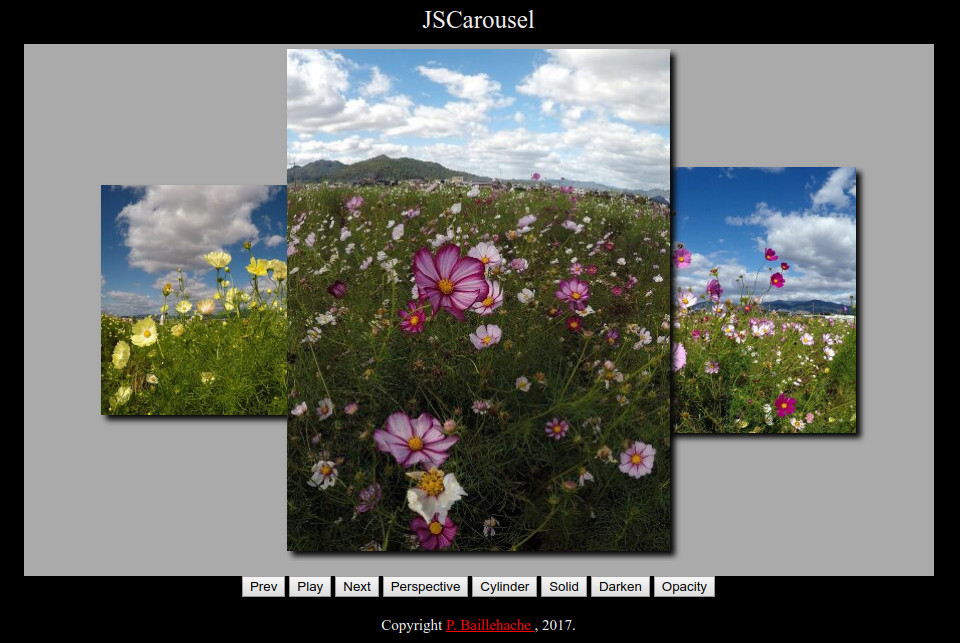
\includegraphics[width=12cm]{jscaroussel.jpg}
\end{center} 


\end{document}


